\ifx\allfiles\undefined
\documentclass{XDBAthesis}
\begin{document}

\def\pictures{}
\else
\fi
\chapter{经典图搜索算法}
\label{chap:classic}
本章将详细介绍几种经典的图搜索算法。由于图搜索算法中大多数采用“过滤-验证”这一框架,所以要提高查询效率,只能从两方面优化。一是在过滤阶段优化,二是在验证阶段优化。众所周知,图是结构化的数据,目前并没有一个统一高效的索引机制可以实现较好的查询结果。所以在过滤阶段,大量学者在研究不同的索引机制,力图通过优化索引的构建和查询来得到更好的查询结果。而在验证阶段,由于子图同构会消耗大量的时间,所以也是个优化的好思路。但是由于子图同构是个NP-hard问题,优化起来并不简单。如何快速检测同构,或将同构转为其他非复杂多项式的一般问题也是学者们关心的一个热点课题。由于本文主要在过滤阶段进行优化,所以本章将介绍的几种查询方法也均为在过滤阶段优化的算法。
\section{图精确搜索算法}
本节将详细介绍精确搜索中的\emph{GraphGrep}算法\cite{graphgrep}和\emph{gIndex}算法\cite{gIndex}。
\subsection{GraphGrep算法}
2002年ShaSha教授等人提出了\emph{GraphGrep}算法\cite{graphgrep} 。GraphGrep算法是基于特征索引方法中的第一个经典算法,它采取典型的“过滤-验证”框架,并只讨论了过滤阶段。由于传统基于结构的算法中需要对图进行顺序遍历比对,其时间空间代价都太高,因此GraphGrep提出了一种基于路径索引和哈希快速存储的过滤方法,来减少候选集大小。

其算法的主要流程是这样的:
\begin{enumerate}
    \item 构造索引:首先将节点和边利用哈希存成两个二维表作为未来筛选用特征之一,然后枚举图数据库中所有长度不大于$l_p $的路径$v_0 ,v_1 ,v_2 ,...,v_k ,( k\leq l_p ,\forall i\in [1,k-1],(v_i ,v_i+1)\in E) $,然后将这些路径与图的关系存为一个二维表作为索引。表的每一行代表每一个图,每一列为一个路径,利用简单哈希确定路径对于行号,每一个单元格代表在该图包含该路径几条,如表\ref{tb:grepIndex}所示。

\begin{table}[htb]
    \centering
    \begin{tabular}{|c|c|c|c|}
        \hline
        Key&$g_1 $&$g_2 $&$g_3 $ \\ \hline
        h(CA)&1&0&1 \\ \hline
        ...&&&\\ \hline
        h(ABAB)&2&2&0 \\
        \hline
    \end{tabular}
    \caption{GraphGrep索引}
    \label{tb:grepIndex}
\end{table}

    \item 解析查询: 如同图数据库,首先将节点和边利用哈希存成两个二维表,然后枚举查询中的所有长度不大于$l_p $的路径,哈希存在一个列表中。
    \item 数据库过滤: 
        \begin{enumerate}
            \item 利用节点信息过滤:如果查询图中的某一节点在数据库中一图里未出现,则此图一定不会包含查询图,因此可以删去。
            \item 利用边信息过滤:同节点过滤,如果某条边未出现,则一定不会包含查询图,可删去。
            \item 利用路径个数进行过滤:如果查询图中某一路径个数大于数据库中一图的此路径个数,则此图一定不会包含查询图,可以从候选集中删去。
        \end{enumerate}
    \item 子图查询: 利用标号进行路径合成,从候选集中删去所有未能成功合成的候选图。剩下的就是GraphGrep算法返回的候选集。后续再加以图同构验证即可得到最终精确搜索结果。
\end{enumerate}
由于GraphGrep算法是基于路径的,编写十分简单,但是路径数目过多,造成索引集很大,建立十分费时,搜索过程中对路径的操作也有大量运算量,尤其在内存有限的情况下哈希常发生冲突现象,因此效果有限。


\subsection{gIndex算法}
2004年,Yan教授等人提出了\emph{gIndex}算法\cite{gIndex}。gIndex是一种以频繁子结构作为索引特征的精确搜索算法。 它采用\emph{动态支持度(size-increasing support)}和\emph{区分度片段}两种方法来优化算法,获得性能更好的索引。

其算法主要流程如此:
\begin{enumerate}
    \item 利用数据挖掘中的相关算法挖掘出频繁子结构,并用最小支持阀值$min\_sup$筛选出频繁子结构作为特征片段
    \item 利用DFS序列化编码将特征片段序列化,然后存成一颗前缀树称为$gIndex$树作为索引,如图\ref{fg:gIndex}所示。并记录每个图包含哪些特征片段。
    \item 对于给定查询图$q$,找出其所有特征片段,然后对包含此片段的图取交集即为最终结果。
\end{enumerate}
\begin{figure}[htb]
    \centering
    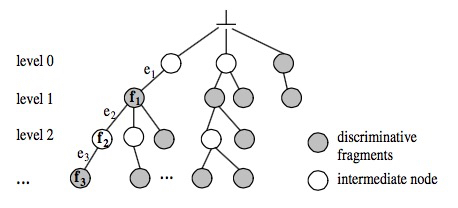
\includegraphics[width=\textwidth ]{../figures/gIndex}
    \caption{gIndex树}
    \label{fg:gIndex}
\end{figure}

gIndex算法是首个以频繁子结构为索引特征的经典算法,其利用了图的结构化信息,使得效率大大提高。但是由于记录的为结构化的子图信息,对空间要求较大,同时特征片段的筛选使得其只携带了自身的结构特点,丢失掉的结构信息也会对算法效率造成一定影响。

\section{图相似性搜索}
本节将着重介绍两种相似性搜索方法,分别是\emph{G-Hash}算法\cite{ghash}和\emph{C-tree}算法\cite{C-Tree}。
\subsection{G-Hash算法}
\emph{G-Hash}算法是Wang教授等人于2009年提出的一种图相似性搜索方法。相比较其他近似搜索方法,这种方法更加稳定高效。G-Hash开创性地采用了\emph{简化包表示(Reduced Bag Represent)}来表示每个节点特征。将图分解成字符串用Hash存储在内存里作为索引。并利用\emph{小波匹配核函数(Wavelet Graph matching kernels)}来计算节点间的相似度,从而得到和查询图最为相似的K个图。但是G-Hash算法的准确度和速度完全取决于相似度度量函数,因此一个好的相似性度量方法尤为重要。

算法主要流程如下:
\begin{enumerate}
    \item 索引构建:将图数据库中每幅图用简化包表示,然后将每个节点特征变为字符串,利用Hash存成索引。如例\ref{ep:ghash_index}所示,就是一个图建成索引过程。需要注意的是在例子中,我们只有三个标号,所以特征矩阵只有四列。但是在实际中当我们选取节点标号数目作为特征时,需要先统计出图数据库中有的所有标号,这样才好做归一化存储。
    \item 查询过程:将查询图也同数据库中图一样用简化包表示。然后计算其中每个节点字符串和图数据库中每个字符串的相似性,乘以每个图中此字符串出现的次数,得到这个节点和每幅图的相似度,求和即可得到总的相似度。排序得到最相近的K个。    
\end{enumerate}

如图\ref{fg:gHashExample},便是G—Hash查询的一个完整例子。
\begin{figure}[htb]
    \centering
    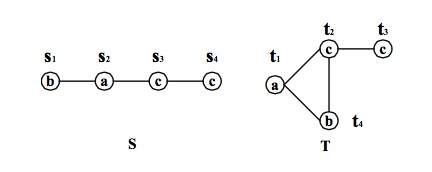
\includegraphics[width=0.7\textwidth ]{../figures/ghashdatabase}
    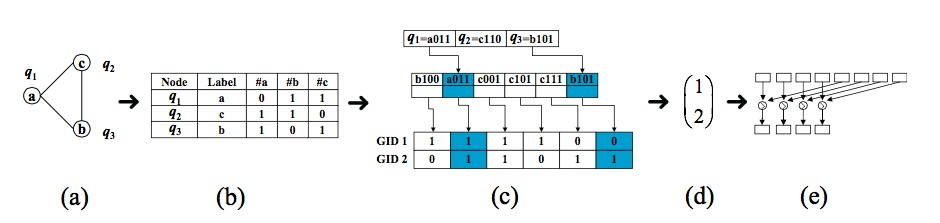
\includegraphics[width=\textwidth ]{../figures/gHash+}
    \caption{G-Hash查询示例:(a)图数据库{S,T}和查询Q,(b)查询Q的简化包表示,(c)与哈希存储的图数据库匹对,(d)计算匹对结果,(e)排序得出最相似的k个图}
    \label{fg:gHashExample}
\end{figure}
\begin{exmp}
        图\ref{fg:ghash_index}就是一个G-Hash构建索引的实例。图\ref{fg:ghash_index}(a)是需要存储的一幅图。我们选取节点标签和邻接节点各个标号的个数作为度量特征,所以一共有四个特征。首先统计各个节点周围各个标号的数目,结果如图\ref{fg:ghash_index}(b)所示 。然后用小波函数提取出实际特征值。举例而言,对于$v_{3}$在用$h=0$的小波函数提取后,局部特征是$\lbrack B,2,0,1\rbrack $。将这些表示特征值的字符串利用Hash找到对应位置,然后将对应节点标号填到此位置,最后生成的哈希表如图\ref{fg:ghash_index}(c)所示。而整个数据库生成的哈希表就如图\ref{fg:ghash_index}(d)所示。
        \label{ep:ghash_index}
        
    \end{exmp}
    
    \begin{figure}[htb]
            \subfigure[一个简单图P]{   
                \begin{minipage}{0.5\textwidth}
                    \centering
                    \ifx\pictures\undefined
\documentclass{article}
\usepackage{ctex}
\usepackage{tikz}
\begin{document}
\else
\fi
\ifx\hasdraw\undefined
\tikzstyle{vertex}=[circle,draw=black!25,minimum size=20pt,inner sep=0pt]
\tikzstyle{edge} = [draw,thick,-]
\def\hasdraw{}
\fi
\begin{tikzpicture}[scale=1.1, auto,swap]
    \foreach \pos/\labels/\name in {{(0,1)/1/A}, {(1,2)/2/A}, {(1,0)/3/B},{(3,0)/4/C}, {(3,2)/5/C}}
        \node[vertex] (\labels) at \pos [label=above:$v_{\labels}$]{$\name$};
    \foreach \source/ \dest  in {1/2,1/3,1/3,2/5,3/4}
            \path[edge] (\source) --  (\dest);
\end{tikzpicture}
\ifx\pictures\undefined
\end{document}
\fi
                \end{minipage}
            }
            \subfigure[节点特征矩阵]{
                \begin{minipage}{0.5\textwidth}
                \centering
                \begin{tabular}{c|c|c|c|c}
                    Nodes & Label & \#A & \#B & \#C \\ \hline
                    $v_{1}$ & A & 1 & 1 & 0 \\ \hline
                    $v_{2}$ & A & 1 & 1 & 1 \\ \hline
                    $v_{3}$ & B & 2 & 0 & 1 \\ \hline
                    $v_{4}$ & C & 0 & 1 & 0 \\ \hline
                    $v_{5}$ & C & 1 & 0 & 0 \\ \hline
                \end{tabular}
            \end{minipage}
            }
            \subfigure[图P对应的哈希表]{
            \begin{minipage}{0.5\textwidth}
                \centering
                \begin{tabular}{c|c}
                    索引键 & 哈希值  \\ \hline
                    A,1,1,0 & $v_{1}$ \\ \hline
                    A,1,1,1 & $v_{2}$ \\ \hline
                    B,2,0,1 & $v_{3}$ \\ \hline
                    C,0,1,0 & $v_{4}$ \\ \hline
                    C,1,0,0 & $v_{5}$ \\ \hline
                \end{tabular}
            \end{minipage}
            }
            \subfigure[图数据库哈希表示例]{
            \begin{minipage}{0.5\textwidth}
                \centering
                \begin{tabular}{c|c|c|c}
                    索引键 & $G_1$ & $G_2$ & $G_3$  \\ \hline
                    A,1,1,0 & 1 & 4 & 0 \\ \hline
                    A,1,1,1 & 0 & 1 & 0 \\ \hline
                    B,2,0,1 & 2 & 0 & 6 \\ \hline
                    C,0,1,0 & 0 & 5 & 1 \\ \hline
                    C,1,0,0 & 3 & 0 & 1 \\ \hline
                \end{tabular}
            \end{minipage}
            }
            \caption{一幅简单示例图}
            \label{fg:ghash_index}
        \end{figure}     


G-Hash算法作为经典的相似性搜索算法,其提出利用核函数计算相似度,成功将结构化特征用数学方法转为数值特征,使得搜索效率有明显提升。但是由于其对哈希函数要求严格,造成编码复杂,而核函数的计算也很耗时,使得此方法实际运用并不多。

\subsection{Closure tree算法}
2006年He和Singh提出了一种基于树结构建立索引的查询算法C-Tree\cite{C-Tree},C-Tree利用启发式图映射方法来判断编辑距离,进而得到近似图。C-Tree具有以下几个特点\cite{DTS}:(1)每个节点都是其孩子的闭包图,只有作为叶子节点的孩子节点是数据库中的图数据;(2)除了根节点每个节点至少包含$m$个孩子$m\geq 2$;(3)每个节点最多不超过$M$个孩子,$(M+1)/2\geq m$。

C-Tree提出了一种利用图闭包计算编辑距离的方法,提出了邻接子树和邻接子图在相似性搜索中的应用,是图相似性搜索领域一个重要基础算法。但是基于图闭包的计算还是略显复杂,仍须研究。

\ifx\allfiles\undefined
\bibliographystyle{unsrt}
\bibliography{main}
\end{document}
\fi